\documentclass[letterpaper,landscape,9pt,fleqn]{extarticle}
%\usepackage[utf8]{inputenc}
%\usepackage[T1]{fontenc}

 \usepackage{pgfplots}

\usepackage{graphicx}
\usepackage{xcolor}
\usepackage{tikz}
\usepackage{url}
\usepackage{qrcode}
%\usetikzlibrary{shapes.geometric}
%\usetikzlibrary{calc}
%\usepackage{fourier}
\usepackage{graphicx,nicefrac}
\usepackage{isomath,upgreek,xcolor,comment}
\usepackage{pdfpages}
%\usepackage{tkz-euclide}
%\usetkzobj{all}
\pagestyle{empty}
\usepackage[activate={true,nocompatibility},final,tracking=true,kerning=true,factor=1100,stretch=10,shrink=10]{microtype}
\usepackage[american]{babel}
\usepackage{centernot}
\usepackage{amstext} % for \text macro
\usepackage{array}   % for \newcolumntype macro
\newcolumntype{L}{>{$}l<{$}} % math-mode version of "l" column type

\newcommand{\dom}{\mathrm{dom}} 
\newcommand{\range}{\mathrm{range}} 
\newcommand{\codom}{\mathrm{codom}}
\newcommand{\zero}{\mathrm{zero}} 
\newcommand{\reals}{\mathbf{R}} 
\newcommand{\ball}{\mathrm{ball}}
\newcommand{\integers}{\mathbf{Z}} 
\newcommand{\ssep}{\mid}
\newcommand{\arcsec}{\mathrm{arcsec}}
\newcommand{\arccsc}{\mathrm{arccsc}}
\newcommand{\arccot}{\mathrm{arccot}}
\newcommand{\glb}{\mathrm{glb}}
\newcommand{\lub}{\mathrm{lub}}
\newcommand{\length}{\mathrm{length}}
\newcommand{\euler}{\mathrm{e}}
\usepackage{mathtools}
\DeclarePairedDelimiter{\parens}{\lparen}{\rparen}
\usepackage{amsmath,amssymb,textcomp}
\everymath{\displaystyle}

%\usepackage{times}
%\renewcommand\familydefault{\sfdefault}
%\usepackage{tgheros}
%\usepackage[defaultmono,scale=0.85]{droidmono}
%\usepackage{fourier}
\usepackage{multicol}
\setlength{\columnseprule}{0pt}
\setlength{\columnsep}{20.0pt}

\usepackage[]{enumerate}
\usepackage{expdlist}

\newenvironment{alphalist}{
  \begin{enumerate}[(a)]
    \addtolength{\itemsep}{-1.0\itemsep}}
  {\end{enumerate}}

\usepackage{geometry}
\geometry{letterpaper,left=0.4in,right=0.4in,top=0.4in,bottom=0.4in}

%\linespread{1.3}


% custom title
\makeatletter
\renewcommand*{\maketitle}{%
\noindent
\begin{minipage}{0.4\textwidth}

\begin{tikzpicture}
\node[rectangle,rounded corners=6pt,inner sep=10pt,fill=blue!50!black,text width= 0.95\textwidth] {\color{white}\Huge \@title};
\end{tikzpicture}
\end{minipage}
\hfill
\begin{minipage}{0.55\textwidth}

\begin{tikzpicture}
\node[rectangle,rounded corners=3pt,inner sep=10pt,draw=blue!50!black,text width= 0.95\textwidth] {\LARGE \@author};
\end{tikzpicture}
\end{minipage}
\bigskip\bigskip
}%
\makeatother

% custom section
\usepackage[explicit]{titlesec}
\newcommand*\sectionlabel{}
\titleformat{\section}
  {\gdef\sectionlabel{}
   \normalfont\sffamily\Large\bfseries\scshape}
  {\gdef\sectionlabel{\thesection\ }}{0pt}
  {
\noindent
\begin{tikzpicture}
\node[rectangle,rounded corners=3pt,inner sep=4pt,fill=blue!50!black,text width= 0.95\columnwidth] {\color{white}\sectionlabel#1};
\end{tikzpicture}
  }
\titlespacing*{\section}{0pt}{15pt}{10pt}


% custom footer
%\usepackage{fancyhdr}
%\makeatletter
%\pagestyle{fancy}
%\fancyhead{}
%\fancyfoot[C]{\footnotesize \textcopyright\ \@date\ \ \@author}
%\renewcommand{\headrulewidth}{0pt}
%\renewcommand{\footrulewidth}{0pt}
%\makeatother

\raggedbottom 
\raggedright
%\usepackage{tikz-3dplot}
\begin{document}

%\maketitle

\begin{multicols*}{3}

\section*{Greek characters}
\begin{tabular}{|L | L| L|} \hline
\mbox{Name} & \mbox{Symbol} & \mbox{Typical use(s)} \\ \hline
\mathrm{alpha} & \alpha  & \mbox{angle, constant} \\
\mathrm{beta} & \beta  & \mbox{angle, constant}  \\ 
\mathrm{gamma} & \gamma & \mbox{angle, constant} \\
\mathrm{delta} & \delta  & \mbox{limit definition}\\
\mathrm{epsilon} & \epsilon  \mbox{ or } \varepsilon & \mbox{limit definition} \\
\mathrm{theta}  & \theta  \mbox{ or } \vartheta &\mbox{angle}\\ 
\mathrm{pi} & \pi \mbox{ or } \uppi & \mbox{circular constant} \\
\mathrm{phi} & \phi \mbox{ or } \varphi  & \mbox{angle, constant} \\
\hline
\end{tabular}

\section*{Named sets}
\begin{minipage}[l]{0.15\textwidth}
    \begin{tabular}{|L | L |} \hline 
        \mathrm{empty\,\, set} & \varnothing \\ 
        \mathrm{real\,\, numbers} & \mathbf{R} \\
        \mathrm{ordered \, \, pairs }  & \mathbf{R}^2 \\
        \hline
    \end{tabular}
\end{minipage}
    \begin{minipage}[l]{0.15\textwidth}
        \begin{tabular}{|L | L |} \hline 
            \mathrm{integers } & \mathbf{Z} \\
            \mathrm{positive \,\,  integers } & \mathbf{Z}_{>0} \\ 
            \mathrm{positive \,\, reals} & \mathbf{R}_{>0} \\
            \hline
        \end{tabular}              
\end{minipage}

\section*{Set symbols}
\begin{minipage}[l]{0.15\textwidth}
    \begin{tabular}{|L | L|} \hline
        \mbox{Meaning}  & \mbox{Symbol} \\ \hline
        \mathrm{is \,\, a \,\, member} & \in \\
        \mathrm{subset}       & \subset \\
        \mathrm{intersection} & \cap \\ \hline
        \end{tabular}   
\end{minipage}
\begin{minipage}[l]{0.15\textwidth}
    \begin{tabular}{|L | L|} \hline
        \mbox{Meaning}  & \mbox{Symbol} \\ \hline
        \mathrm{union} & \cup  \\ 
        \mathrm{complement} & \mbox{superscript}^\mathrm{C} \\
        \mathrm{set \,\,  minus}  & \setminus \\ \hline
        \end{tabular}   
\end{minipage}

\section*{Logic symbols}
\begin{minipage}[l]{0.15\textwidth}
    \begin{tabular}{|L | L|} \hline 
        \mbox{Meaning}  & \mbox{Symbol} \\ \hline 
        \mathrm{negation} &  \lnot   \\
        \mathrm{and} &  \land  \\
        \mathrm{or} &  \lor  \\
        \mathrm{implies} &  \implies \\ \hline    
    \end{tabular}   
\end{minipage}
\begin{minipage}[c]{0.15\textwidth}
    \begin{tabular}{|L | L|} \hline 
        \mbox{Meaning}  & \mbox{Symbol} \\ \hline 
        \mbox{equivalent} &  \equiv \\ 
        \mbox{iff} & \iff \\ 
        \mbox{for all} & \forall \\
        \mbox{there exists} & \exists \\ \hline
    \end{tabular}   
\end{minipage}



\section*{Arithmetic properties of \(\reals\)}
\begin{alignat*}{2}
    &\parens*{\forall a,b\in \reals} \parens*{a + b = b + a} & \mbox{commutivity}\\
    &\parens*{\forall a,b,c\in \reals} \parens*{a + (b + c)  = (a+b)+c} & \mbox{associative}\\
    &\parens*{\forall a,b \in \reals} \parens*{a  b = b a} & \mbox{commutivity}\\
    &\parens*{\forall a,b,c \in \reals} \parens*{a  (b c) = (a b) c} & \mbox{associative}\\
    &\parens*{\forall a,b,c \in \reals} \parens*{a (b+c) =a b + a c} & \mbox{distributive}\\
\end{alignat*}

\section*{Intervals}
\begin{minipage}[c]{0.3333333333333\textwidth}
For numbers \(a\) and \(b\), we define the intervals
\begin{align*}
 (a,b) &= \left\{x \in \reals \ssep a < x < b \right\}  \\
  [a,b) &= \left \{x  \in \reals  \ssep a \leq  x < b \right \} \\
   (a,b] &= \left \{x  \in \reals \ssep a <  x \leq  b \right \} \\
    [a,b]  &= \left \{x  \in \reals \ssep a \leq  x \leq  b \right \} \\
 %   (-\infty, a) &= \{x \mid x < a \} \\
 %   (-\infty, a] &= \{x \mid x \leq  a \} \\
 % (a, \infty)  &= \{x \mid a < x  \} \\
 %  [a, \infty)  &= \{x \mid a \leq  x  \} \\
\end{align*}  
\end{minipage}
\vspace{-0.25in}

\section*{Distance \& Midpoint}
\vspace{-0.15in}
\begin{minipage}[c]{0.3333333333333\textwidth}
The distance between the points \((x_1,y_1)\) and  \((x_2,y_2)\) is
\[
  \sqrt{(x_1-x_2)^2 + (y_1-y_2)^2}.
\]
The midpoint is the point
\[
\left(\frac{x_1+x_2}{2}, \frac{y_1+y_2}{2} \right).
\]
\end{minipage}

\section*{Exponents}
\vspace{-0.15in}
\begin{minipage}[c]{0.3333333333333\textwidth}
%\vspace{-0.25in}
For \(a,b > 0\) and \(m,n\) real:
\begin{alignat*}{1}
&a^0 = 1,  \quad \quad 0^a = 0\\
&1^a = 1, \quad \quad  a^n a^m = a^{n+m}  \\
&\nicefrac{a^n}{a^m} = a^{n-m}, \quad \quad (a^n)^m = a^{n \cdot m} \\
&a^{-m} = \nicefrac{1}{a^m}, \quad \quad \left(\nicefrac{a}{b}\right)^m = \nicefrac{a^m}{b^m} 
\end{alignat*}
\end{minipage}

\section*{Radicals}
\begin{minipage}[c]{0.3333333333333\textwidth}
\begin{alignat*}{1}
&\sqrt[n]{a} = a^{1/n} \\
&\sqrt[n]{ab} = \sqrt[n]{a} \sqrt[n]{b}  \quad (\mbox{provided } a,b \geq 0) \\
&\sqrt[m]{\sqrt[n]{a}} = \sqrt[mn]{a} \\
&\sqrt[n]{\frac{a}{b}} = \frac{\sqrt[n]{a}}{\sqrt[n]{b}} \\
&\sqrt[n]{a^n} = \begin{cases} a & n \mbox{ odd} \\  |a| &  n \mbox{ even} \end{cases}
\end{alignat*}
\end{minipage}

\section*{Identities}
\begin{minipage}[c]{0.3333333333333\textwidth}
\begin{alignat*}{2}
   &a  \parens*{b + c} = a b + a c \\
   &\parens*{\parens{a +b}  \parens*{c + d}} = a c + a d + b c + bd \\
   &\frac{a b + ac}{a} = b + c  \quad (\mbox{provided } a \neq 0) \\
   &\frac{\frac{a}{b}}{\frac{c}{d}} = \frac{ad}{b c}  \quad (\mbox{provided } b,d \neq 0) \\
   &\sqrt{a b} = \sqrt{a}\sqrt{b}  \quad (\mbox{provided } a \geq 0, b \geq 0 ) \\
   &\ln(ab) = \ln(a) + \ln(b) \quad (\mbox{provided } a \geq 0, b \geq 0 ) \\
\end{alignat*}
\end{minipage}
\section*{Solution of Equations}
%\vspace{-0.2in}
\subsubsection*{Algebraic}
%\vspace{-0.2in}
\begin{minipage}[c]{0.3333333333333\textwidth}
\begin{align*}
& \big [a b = 0 \big ] \equiv \big [ a = 0 \mbox{ \textbf{or} } b = 0 \big ]\\
& \big [ a^2 = b^2 \big ] \equiv \big [ a = b \mbox{ \textbf{or} } a = -b \big ]\\
&\left [ \frac{a}{b} = 0 \right ] \equiv \big [ a = 0 \mbox{ \textbf{and} } b \neq 0 \big ] \\
&\left [\frac{a}{b} = \frac{c}{d}  \right ] \equiv \big [ad  = bc \mbox{ \textbf{and}  } b \neq 0  \mbox{ \textbf{and}  }  d \neq 0 \big ] \\
&\big [|a| = |b|  \big ] \equiv \big [a =b \mbox{ \textbf{or} } a = -b \big ]\\
&\big [ \sqrt{a}  = b \big ] \equiv \big [a = b^2 \mbox{ \textbf{and}  } b \ge 0 \big ] \\
\intertext{For \(a \neq 0\),}
& \big [a x^2 + b x + c = 0 \big] \equiv \left [x = \frac{-b \pm \sqrt{b^2 - 4 a c}}{2 a} \right] \\
\end{align*}
%\vspace{-0.52in}
\subsubsection*{Exponential}
%\vspace{-0.2in}
\begin{align*}
& \big [\ln(a) = 0 \big] \equiv \big [a =  1\big] \\
& \big [\euler^a = 1 \big] \equiv \big [a = 0 \big] \\
& \big [\ln(a) = b \big] \equiv \big [a = \euler^b \big] \\
\end{align*}
\end{minipage}
\section*{Logarithms}
   \begin{equation*}
  \log_a(x) = \frac{\ln(x)}{\ln(a)}
     \end{equation*}
\vfill

\section*{Graph Translations}
\begin{minipage}[c]{0.3333333333333\textwidth}
For the graph of $F(x,y) = 0$  
\begin{itemize}
 \item The graph of $F(x-h,y)=0$ is the graph of $F(x,y) = 0$ translated $h$ units to the right. 
 
 \item The graph of $F(x,y-k)=0$ is the graph of $F(x,y) = 0$ translated $k$ units up. 
 
 \item The graph of $F(x/c,y)=0$ is the graph of $F(x,y) = 0$ stretched a factor of $c$ horizontally. 
 
 \item The graph of $F(x,y/c)=0$ is the graph of $F(x,y) = 0$ stretched a factor of $c$ vertically.
 \end{itemize}
\end{minipage}

\section*{Circles}
\begin{minipage}[c]{0.3333333333333\textwidth}
Equation of circle centered at $(h,k)$ with radius $r$ is
\[
   (x - h)^2 +  (y - k)^2  = r^2. 
\]
Expanded the equation is
\[
   x^2 - 2h x + y^2 - 2 k y = r^2 - h^2 - k^2. 
\]
\end{minipage}[c]

\section*{Parabolas \& Lines}
\begin{minipage}[c]{0.3333333333333\textwidth}
The vertex of the parabola $a x^2 + b x + c = y$ is
\[
   \left(x = -\frac{b}{2 a}, y = c-\frac{{{b}^{2}}}{4 a} \right).
\]
An equation of the line that contains the points
\( (x_1, y_1) \) and  \((x_2, y_2) \) is
\[
  y - y_1 = \left(\frac{y_2-y_1}{x_2-x_1} \right) (x - x_1).
\]
The number \(\frac{y_2-y_1}{x_2-x_1} \) is the slope.
\end{minipage}




\section*{Function notation}
\begin{tabular}{|L | L|} \hline 
    \dom(F) &   \mbox{domain of function } F \\
    \range(F) &   \mbox{range of function } F \\ \hline
 \end{tabular}

\section*{Domains, Ranges, and Zeros}


\begin{tabular}{|L | L| L | L |} \hline 
 \mathrm{Function}  & \mathrm{Domain} & \mathrm{Range}   &  \mathrm{Zeros} \\ \hline
\ln, \log       & (0,\infty)  &  (-\infty, \infty)  & 1  \\
\exp       &  (-\infty, \infty)   &  (0,\infty)  & \varnothing   \\
\mathrm{abs}        &   (-\infty, \infty)  & (0,\infty) &  0   \\
\sqrt{}        &   (0, \infty)  & (0,\infty) &  0   \\
\sqrt[3]{}       &   (-\infty, \infty)  & (-\infty, \infty) &  0   \\
\mathrm{floor}                  &  (-\infty, \infty)   & \integers & [0,1) \\
\mathrm{ceiling}              &  (-\infty, \infty)  &  \integers   & (-1,0] \\ \hline
\end{tabular}



\section*{Compound Interest}
\begin{minipage}[c]{0.3333333333333\textwidth}
Interest rate $r$ compounded $n$ times
per year
\[  A = P (1 + r/n)^{n t}
    \]
Continuous compounding:
\[
    A = P \euler^{r t}
\]
%\vspace{0.2in}
\end{minipage}

\section*{Exponential Growth}
The exponential function that contains
the points \((t=t_o, y=y_o)\) and \((t=t_1, y=y_1)\)
is
\begin{equation*}
    y = y_o \parens*{\frac{y_1}{y_o}}^{\frac{t-t_o}{t_1-t_o}}.
\end{equation*}


 
%\vfill 
\section*{Graphs}
Graph of natural logarithm
%\vspace{0.1in}
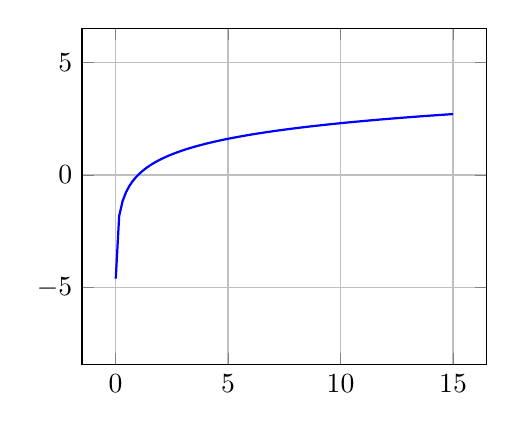
\begin{tikzpicture}
        \begin{axis}[domain=0.01:15,
            samples=100,
            grid=both,
            scale=0.75,
            no markers,
            axis equal]
        \addplot +[thick] {ln(x)};
       % \addplot +[thick, domain=0:5] {ln(2)};
       % \addplot +[thick, dashed] coordinates {(1,0)(1,4)};
        \end{axis}
    \end{tikzpicture} \\
    
   Graph of natural exponential
%\vspace{0.1in}
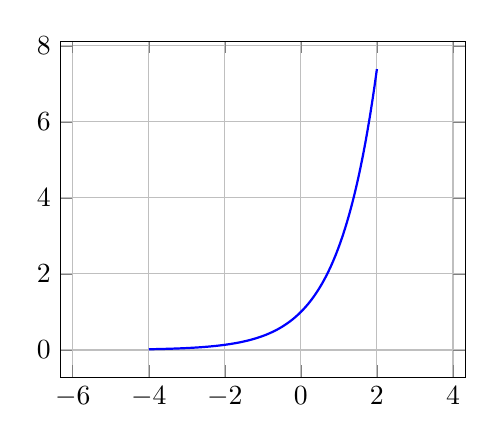
\begin{tikzpicture}
        \begin{axis}[domain=-4:2,
            samples=100,
            grid=both,
            scale=0.75,
            no markers,
            axis equal]
        \addplot +[thick] {exp(x)};
       % \addplot +[thick, domain=0:5] {ln(2)};
       % \addplot +[thick, dashed] coordinates {(1,0)(1,4)};
        \end{axis}
    \end{tikzpicture}
  %  \caption{Graph of $y = \ln(x)$}

% See https://www.stat.rice.edu/~dobelman/notes_papers/math/Cheatsheet.Maths.pdf
% I like the common errors

\section*{Common Errors}
\begin{tabular}{|L | L|} \hline
\mbox{\textbf{Error}} & \mbox{\textbf{Correct or Example}}  \\ \hline
\nicefrac{x}{0}=0 \mbox{ or } x  & \nicefrac{x}{0} \mbox{ is undefined} \\
-x^2 = x^2       & -x^2 = -(x^2) \\ 
\nicefrac{a}{(b+c)} = \nicefrac{a}{b} + \nicefrac{a}{c} &  \nicefrac{1}{(1+1)} \neq \nicefrac{1}{1} + \nicefrac{1}{1}\\ 
\nicefrac{a+b x}{a} = 1+ b x  & \nicefrac{a+b x}{a} = 1+\nicefrac{b x}{a} \\
\parens*{a+b}^2 = a^2 + b^2 & \parens*{a+b}^2 = a^2+2 a b + b^2 \\
\sqrt{a+b} = \sqrt{a} + \sqrt{b} &  \sqrt{1+1} \neq \sqrt{1} + \sqrt{1}\\  \hline

  \end{tabular}

\vfill
\noindent {\textbf{Revised} \today by Barton Willis. This work is
licensed under Attribution 4.0 International (CC BY 4.0) \,  \qrcode[height=0.15in]{https://creativecommons.org/licenses/by/4.0/}. For the current version of
this document, visit \, \qrcode[height=0.15in]{https://github.com/barton-willis/College-algebra}}
\end{multicols*}%{3}

\end{document}